% Ajustement, taux d'évolution et tableur, suite géométrique

\section{Dépenses de santé (7 points)}

Le tableau suivant, extrait d'une feuille d'un tableur, donne la consommation de soins et de biens médicaux en milliards d'euros depuis l'année 2000.

\begin{center}
	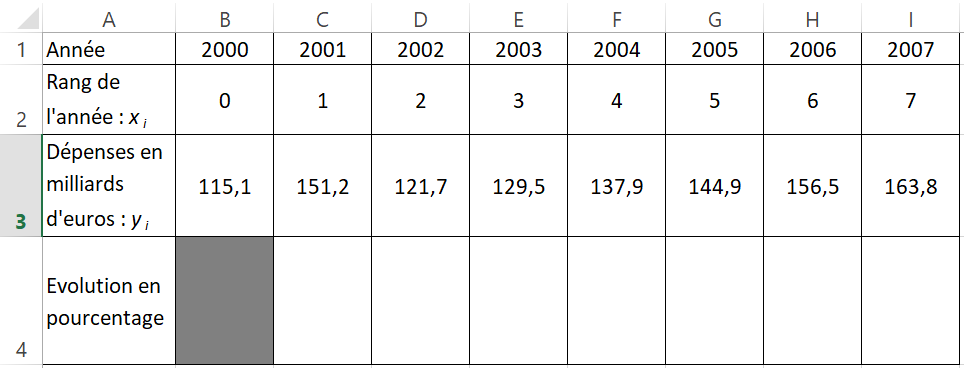
\includegraphics[scale=0.65]{img/biens_medicaux2}
\end{center}

\emph{Il n'est pas demandé de compléter le tableau.}

\subsection{Droite d'ajustement}

\begin{questions}
	\question[1] On suppose que la droite d'ajustement entre le rang de l'année $x$ et les dépenses en milliards d'euros $y$ a pour équation : $y = 7x + 115$. En utilisant cette équation, déterminer le montant des dépenses en 2010. 
	\begin{solution}
		L'année 2000 correspond au rang 0, donc le rang de l'année 2010 est 10. Calcul du montant des dépenses en 2010 :
		\begin{eqnarray*}
			y &=& 7x + 115 \\
			y &=& 7 \times 10 + 115 \\
			y &=& 185
		\end{eqnarray*}
	
	D'après l'équation de la droite d'ajustement, en 2010 les dépenses s'élèveront à 188 milliards d'euros.
	\end{solution}

\end{questions}

\subsection{Pourcentage d'évolution}

\begin{questions}
	\question[1] Quel est le pourcentage d'évolution global entre 2000 et 2007, à \num{0.1} \% prês ? 
	\begin{solution}
		\begin{eqnarray*}
			t &=& \dfrac{valeur d'arrivée - valeur de départ}{valeur de départ} \\
			t &=& \dfrac{\num{163.8} - \num{115.1}}{\num{115.1}} \\
			t &=& \dfrac{\num{48.7}}{\num{115.1}} \\
			t &=& \num{0.423}
		\end{eqnarray*}
	
		Soit une augmentation de \num{42.3} \% du montant des dépenses entre 2000 et 2007.
	\end{solution}

	\question[1] Quelle formule doit-on entrer en $C4$ pour déterminer le taux d'évolution des dépenses entre 2000 et 2001 et pouvoir la recopier vers la droite jusqu'en $I4$ ?
	\begin{solution}
		Pour déterminer le taux d'évolution des dépenses entre 2000 et 2001 il faut saisir la formule suivante en $C4$  :
		\begin{equation*}
			= (C3 - B3) / B3
		\end{equation*}
	\end{solution}
\end{questions}

\subsection{Limitation des dépenses}

Afin de mieux maîtriser les dépenses de santé, le gouvernement souhaitait, à partir de 2008, que les dépenses liées à la consommation de soins et de biens médicaux n'augmentent que de 2 \% par année. On modélise cette évolution par une suite. On désigne par $u_n$ le montant maîtrisé des dépenses pour l'année (2007 + $n$) en milliards d'euros. On a donc $u_0 = \num{163.8}$.

\begin{questions}
	\question[1] Calculer la valeur de $u_1$ (donner la valeur exacte).
	\begin{solution}
		Calcul de la valeur $u_1$ :
		\begin{eqnarray*}
			u_1 &=& u_O + \dfrac{u_0 \times 2}{100} \\
			u_1 &=& \num{163.8} + \dfrac{\num{163.8} \times 2}{100} \\
			u_1 &=& \num{163.8} + \num{3.276} \\
			u_1 &=& \num{167.076}
		\end{eqnarray*}
	\end{solution} 
	
	\question[1] Quelle est la nature de la suite $(u_n)$ ? On précisera les éléments caractéristiques de la suite.
	\begin{solution}
		Les dépenses liées à la consommation de soins et biens médicaux augmente de 2\% par an, donc chaque terme de la suite est obtenu est obtenu en multipliant le précédent par \num{1.02}.
		J'en déduis que $(u_n)$ est une suite géométrique de premier terme $u_0=\num{163.8}$ et de raison $q=\num{1.02}$.
	\end{solution}
	
	\question[1] Exprimer $u_n$ en fonction de $n$.
	\begin{solution}
		Expression de $u_n$ en fonction de $n$ :
		\begin{eqnarray*}
			u_n &=& u_0 \times q^n \\
			u_n &=& \num{163.8} \times \num{1.02}^n 
		\end{eqnarray*}
	\end{solution}
	
	\question[1] En supposant que cette modélisation reste valable jusqu'en 2015, à combien peut-on estimer le montant des dépenses en 2015 ? (Le résultat est à arrondir à $10^{-3}$).
	
	\begin{solution}
				
		$2015 = 2007 + 8$, donc pour estimer le montant des dépenses en 2015 il faut calculer la valeur du huitième terme de la suite, $u_8$ :
		
		\begin{eqnarray*}
			u_8 &=& \num{163.8} \times \num{1.02}^8 \\
			u_8 &\approx&  \num{191.918}\\
		\end{eqnarray*}
		
		On peut donc estimer le montant des dépenses en 2015 à  \num{191.918} milliards d'euros.
	\end{solution}
\end{questions}

  